%% ==============================
\chapter{Methods}
\label{sec:methods}
%% ==============================
The general methodology of this work follows an iterative design principle. First, related work with specific approaches was analyzed. These approaches used benchmark environments to test their implementation and compare it to previous approaches. These benchmarks were used as a starting point for the development of the planner for this work. In the first evaluation phase, the developed planner was compared to other algorithms on the same benchmarks. A new metric was developed to quantify the disturbance of the public space. In the next step, the hierarchical planner was tested on a model of a real building. To combine these concepts, they were integrated into the \gls{nav_2} stack and tested in a simulated hospital environment. Throughout these steps, the code was continuously improved and debugged.

A limitation of the methodology of his work is that no comparative evaluation of the developed hierarchical planner with related work has been performed. This is due to the fact that the focus of this work is the implementation on a real robot with ROS 2, unlike older approaches that used different frameworks and did not publish the code online as open source. Also, the optimization of the developed planner in terms of computational speed was not the scope of this work. As a result, direct comparisons of planning times and other metrics of the hierarchical planner are lacking. A comparison of the straight path planner was performed as described in the following sections.

%% ==============================
\section{Existing Benchmarks}
\label{sec:benchmarks}
%% ==============================
 As seen in the literature review in Chapter \ref{sec:state_of_the_art}, most related works used common benchmarks to test their approaches. Specifically, the benchmark from \cite{ryu_hierarchical_2020} was used to test hierarchy creation and two-level hierarchical planning. This environment is a map of a real building. It was originally recorded by Stachniss \cite{cyrill_stachniss_robotics_2015} on the campus of the University of Freiburg, see Figure \ref{fig:freiburg_benchmark}. The second benchmark environment was previously shown in Figure \ref{fig:htm_global_comparison} and is mainly used to compare the straight path planner with the previous approaches. It was also used by Hou et al. \cite{hou_straight_2021} with the SIRRT* planner and by Beeson et al. \cite{beeson_towards_2005} with the EVG planner.

\begin{figure}[h]
    \centering
    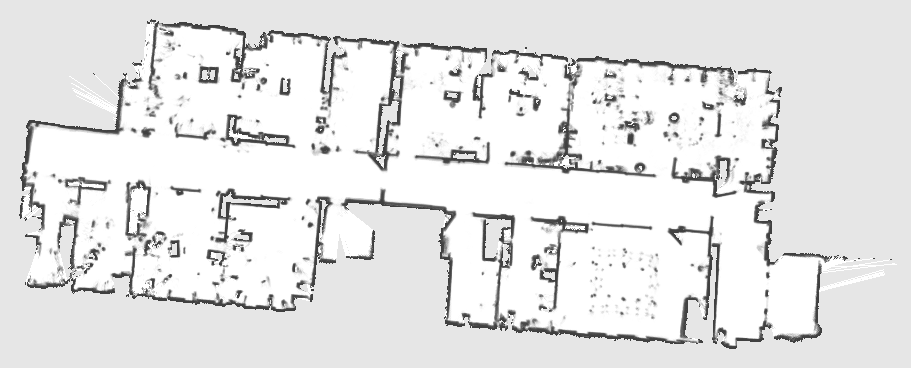
\includegraphics[width=0.75\textwidth]{figures/30_methods/freiburg_benchmark.png}
    \caption[The benchmark environment for hierarchy creation and straight path planning]{The benchmark environment for hierarchy creation and straight path planning recorded in the University of Freiburg (Source: \cite{cyrill_stachniss_robotics_2015})}
    \label{fig:freiburg_benchmark}
\end{figure}

In the first evaluation phase of the iterative process, the developed straight path planner is tested on these benchmark environments and compared to related work and common path planner algorithms. To ensure reliable and statistically significant results, each planner is tested on different benchmarks and the corresponding submaps of a single room. Each planner produces a number of paths resulting from the number of combinations of start and goal positions. These positions consist of \(n_r\) randomly sampled points in the drivable area and all bridge points \(n_b\) of the environment or submap. The total number of paths \(n_{\text{paths}}\) results from selecting two of these points from the start and goal points and repeating this for all possible combinations. This can be expressed by the binomial coefficient formula, where \(k\) is 2 because there is only one start point and one goal point, see the Equation \ref{equ:binomial_coefficient}.
\begin{equation} \label{equ:binomial_coefficient}
    n_{\text{paths}} = \binom{n_r + n_b}{2} = \frac{(n_r + n_b)!}{2! ((n_r + n_b)-2)!}
\end{equation}
In the case of one example room, there are 3 bridge points \(n_b\) and an additional 10 random points \(n_r\), resulting in 78 paths. In the case of the complete floor from the benchmark in Figure \ref{fig:freiburg_benchmark} \(n_b = 27\) and \(n_r = 20\), resulting in 1081 paths. These paths were then evaluated using the following metrics:
\begin{enumerate}
    \item \textbf{Success Rate}: Percentage of valid paths found
    \item \textbf{Path Length}: Total length from start to goal in pixels
    \item \textbf{Planning Time}: Total planning time including smoothing
    \item \textbf{Path Smoothness}: Sum of deviation angles divided by path length
    \item \textbf{Obstacle Clearance}: Mean distance from path to obstacles
    \item \textbf{Distance Deviation}: Standard deviation of distance between path and obstacles
    \item \textbf{Distance to Centroid}: Mean distance of the path to the centroid of the room
    \item \textbf{Disturbance of Public Space}: Largest open area within the map divided by total room area (details in Chapter \ref{sec:new_metric})
\end{enumerate}

%% ==============================
\section{New Metric for Disturbance of Public Space}
\label{sec:new_metric}
%% ==============================
The problem statement in Chapter \ref{sec:problem_statement} presents the need for straight, deterministic, and predictable paths. In certain situations, it is important to drive close to the walls and not directly across the room. Such a scenario is shown in Figure \ref{fig:straight_path_problem}. In order to measure the planner's ability to produce paths that by design have little impact on the public space, a new metric must be invented. So far, there is no such metric in the literature because most path planning problems focus on finding the shortest possible solution. In contrast, this work focuses on straight paths and predictability. To avoid driving directly through a major human traffic route or through the queue of an information desk, this planner tries to stay close and parallel to the walls. This new metric provides a way to quantify this behavior. Unlike most path metrics and all of the metrics mentioned in the previous chapter, this new metric cannot be calculated from a single solution path. It gives a value for how well all possible paths in the map combined avoid the public space. The process of obtaining this value for one single room is described in the following:

\begin{enumerate}
    \item Get all bridge points \(n_b\) connecting this room to neighboring rooms or other hierarchies.
\item Sample \(n_r\) random points within the valid area (default \(n_r = 10\))
    \item Plan paths for all possible connections given by the equation \ref{equ:binomial_coefficient}
    \item Overlay all paths on the original room environment \(R\)
    \item Segment the room into connected components \(CC_{\text{free}}\) that are not separated by paths
    \item Get the largest connected components by area \(CC_{\text{free, max}} = \max \{\text{area}(CC_{\text{free}})\}\)
    \item Divide by the total area of the room and subtract from 1 to get the disturbance value \(D\) as in the equation \ref{equ:disturbance}.
\end{enumerate}
\begin{equation}
\label{equ:disturbance}
    D = 1 - \frac{\max \{\text{{area}}(CC_{\text{{free}}})\}}{{\text{{area}}(R)}}
\end{equation}

This results in a metric measuring public space disturbance for a single room, where a low value indicates desirable behavior for a mobile robot. Figure \ref{fig:disturbance_example} shows a comparison of the metric on a room from the second benchmark.

\begin{figure}[h]
    \captionsetup[subfigure]{justification=centering}
    \centering
    \begin{subfigure}{.5\textwidth}
      \centering
      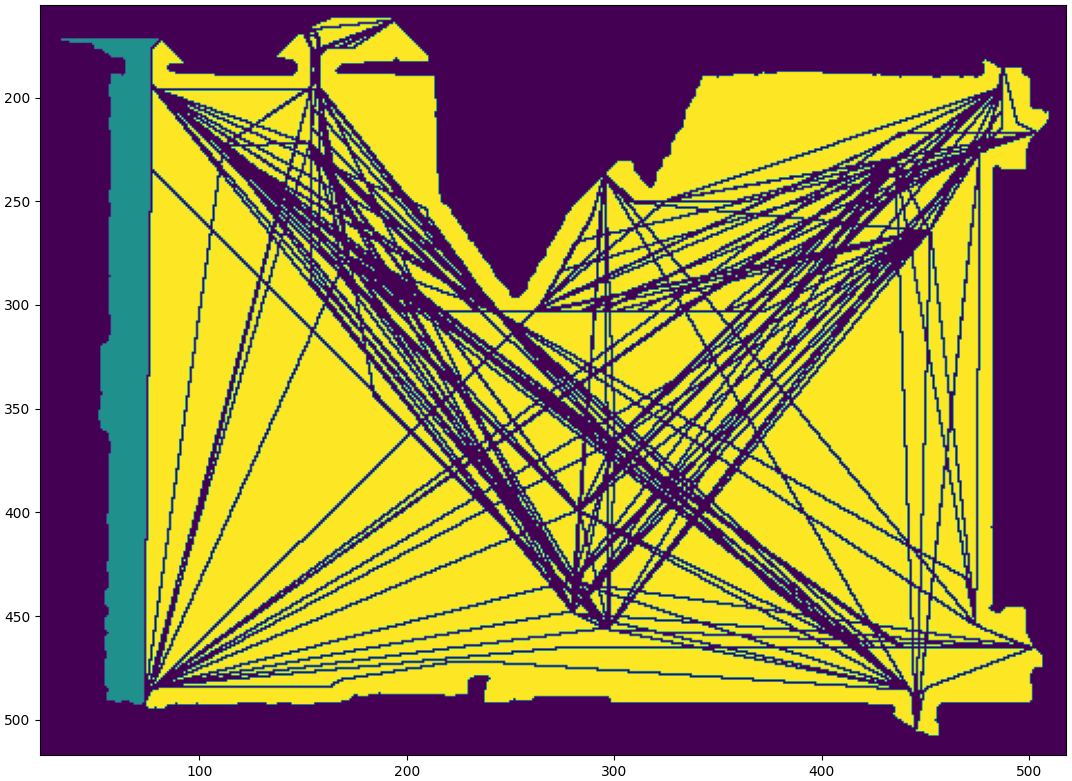
\includegraphics[width=\textwidth]{figures/30_methods/room9_disturbance_astar_smooth.png}
      \caption{Planner: A*, \(D = 0.95\)}
    \end{subfigure}%
    \begin{subfigure}{.5\textwidth}
      \centering
      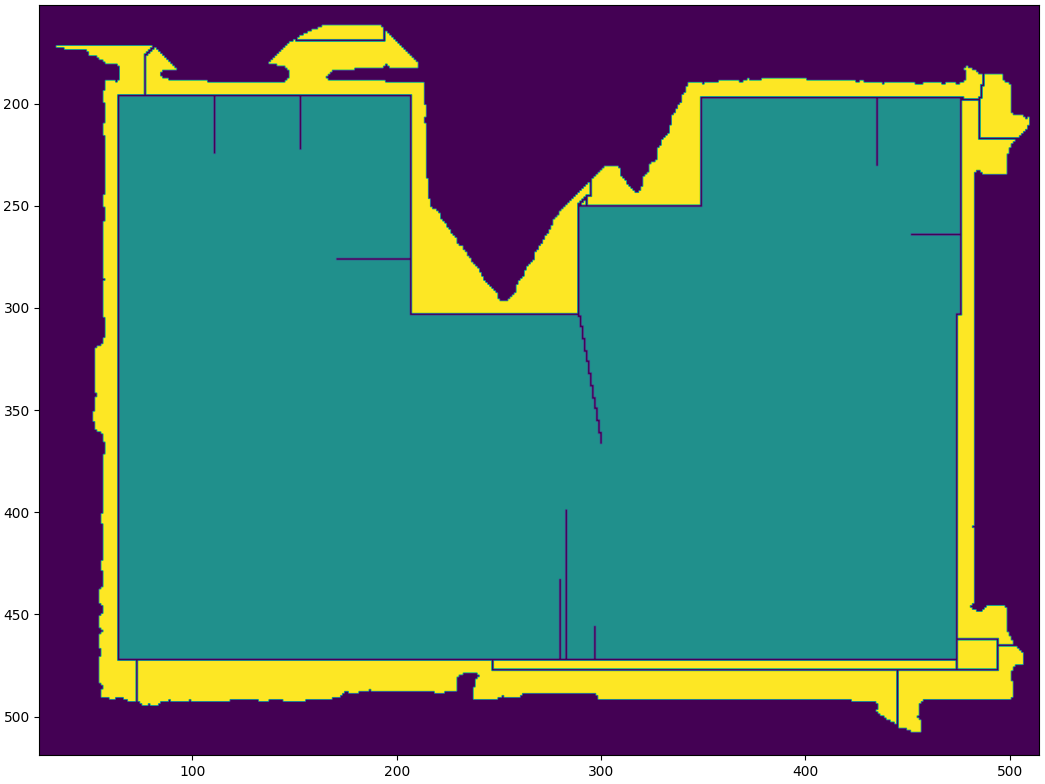
\includegraphics[width=.975\textwidth]{figures/30_methods/room9_disturbance_ilir_smooth.png}
      \caption{Planner: ILIR, \(D = 0.20\)}
    \end{subfigure}
    \caption[Example of the metric for disturbance of public space]{Example of the metric for the disturbance of public space with \(n_r=10\), \(n_b=9\), \(n_{\text{paths}}=171\). The area of the original room \(R\) in yellow and turquoise, the paths and walls in purple and the largest free area \(CC_{\text{free, max}}\) in turquoise.}
    \label{fig:disturbance_example}
\end{figure}

%% ==============================
\section{Simulation}
\label{sec:simulation}
%% ==============================
After developing hierarchy generation and two-level hierarchical planning, a more complex environment was needed to evaluate hierarchical planning with arbitrary hierarchical levels and connections between them. For this purpose, the campus of our research lab was modeled as a graph and used for planning. This environment is complex in terms of hierarchical connections, e.g. some stairs connect the second floor diagonally to the terrace of the first floor, which itself is shaped in a ring connecting all other buildings. This makes this environment more complex than a simple building with a vertical connection through an elevator, as used in previous work such as Gregoric et al. \cite{gregoric_autonomous_2022} or Cagigas \cite{cagigas_hierarchical_2005}. An image of the campus and the corresponding graph can be seen in Figure \ref{fig:ltc_rendering}.

\begin{figure}[h]
    \captionsetup[subfigure]{justification=centering}
    \centering
    \begin{subfigure}{.5\textwidth}
      \centering
      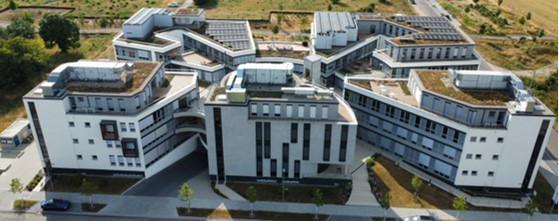
\includegraphics[width=\textwidth]{figures/30_methods/ltc_real.jpg}
      \caption{\gls{iras} campus}
    \end{subfigure}%
    \begin{subfigure}{.5\textwidth}
      \centering
      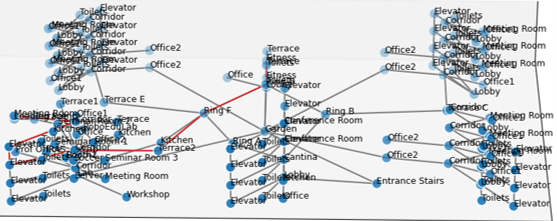
\includegraphics[width=\textwidth]{figures/30_methods/ltc_graph.png}
      \caption{Graph representation}
    \end{subfigure}
    \captionsetup{justification=centering}
    \caption[Image and graph representation of the \gls{iras} research campus]{Image a) and graph representation b) of the \gls{iras} research campus.}
    \label{fig:ltc_rendering}
\end{figure}

Both concepts, the hierarchical planner and the straight path planner, were combined and integrated into the \gls{nav_2} stack for \gls{ros_2}. For quick testing, this was done in a simulated hospital environment. This helps with debugging and accelerates development. The publicly available "AWS RoboMaker Hospital World" from Amazon \cite{aws_robotics_aws_2023} was used. Figure \ref{fig:aws_hospital} shows the simulated hospital. The advantage of this environment is that it also provides models for two and three floors. From this simulation the gap to the real world is small and it can finally be implemented on the real PeTRA robot.

\begin{figure}[h]
    \centering
    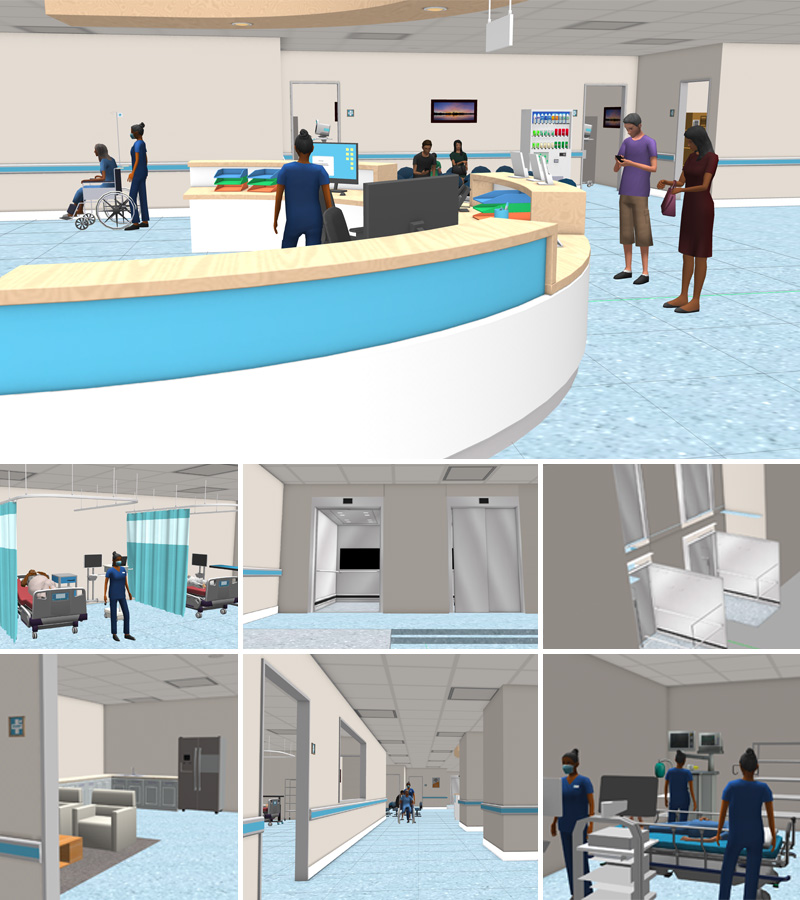
\includegraphics[width=0.5\textwidth]{figures/30_methods/hospital_world.jpg}
    \caption[The "AWS RoboMaker Hospital World" simulation environment for Gazebo]{The "AWS RoboMaker Hospital World" simulation environment for Gazebo. (Source: \cite{aws_robotics_aws_2023})}
    \label{fig:aws_hospital}
\end{figure}